documentclass[]
\usepackage{amsmath}
\usepackage{tikz}
\usetikzlibrary{backgrounds,decorations.pathreplacing,calc,arrows.meta}
\tikzset{
    myarrow/.style={-{Latex[scale=1.5]}},
    myarrowblack/.style={-{Latex[scale=1.5]},color=black},
    }
\begin{document}
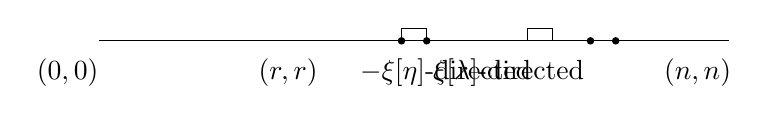
\begin{tikzpicture}[scale=.8]
    \draw (0,0)--(10,0);
    \draw[fill=white] (4.8,0)--(5.2,0)--(5.2,.2)--(4.8,.2)--cycle;
    \draw[fill=white] (6.8,0)--(7.2,0)--(7.2,.2)--(6.8,.2)--cycle;
    \node[] at (-.5,-.5) {$(0,0)$};
    \node[] at (3,-.5) {$(r,r)$};
    \node[] at (9.5,-.5) {$(n,n)$};
    \draw[fill] (4.8,0) circle (.05);
    \draw[fill] (5.2,0) circle (.05);
    \draw[fill] (7.8,0) circle (.05);
    \draw[fill] (8.2,0) circle (.05);
    \node[myarrow] at (6.5,-.5) {$\xi[\lambda]$-directed};
    \node[myarrowblack] at (5.5,-.5) {$-\xi[\eta]$-directed};
    \end{tikzpicture}
\end{document}